\documentclass[11pt]{article}
\usepackage[letterpaper,margin=.72in]{geometry}
\usepackage[T1]{fontenc}
\usepackage{lmodern,microtype,graphicx,booktabs,amsmath,hyperref,xurl}
\hypersetup{colorlinks=true,urlcolor=blue,pdfauthor={James N. Jean IV},pdftitle={Establishment growth signals with an explicit denominator}}
\setlength{\parindent}{0pt}\setlength{\parskip}{6pt}\renewcommand{\arraystretch}{1.08}
\begin{document}
{\Large\bfseries Establishment growth signals with an explicit denominator}\par
James N. Jean IV\hfill 29 October 2026\par
\textit{Independent study 10. Not peer reviewed.}
\section*{Decision brief}
An employment dashboard should distinguish opening activity from expansion at continuing establishments. This study tests whether a simple same-industry pool improves a prior-year baseline for a published expansion-rate proxy, using a fixed state-sector cohort and later calendar years.

A fixed 25\% own-history / 75\% other-state pool has held equal-series MAE 3.125 percentage points versus 3.327 for the own-lag baseline, a 6.1\% reduction across 934 state-sector series and 3,736 annual cases. The selected model is worse in 428 series and four of nineteen sectors, and slightly worse in 2023. All failures remain in the result tables.

The target is a published expansion-rate proxy: job gains at expanding continuing establishments per 100 DHS-average employees in the whole state-sector cell. It is not worker hires, job vacancies or a demonstrated labor shortage. This is a retrospective revised-data comparison; complete prior-year inputs are idealized and original information vintages remain unverified.

Use the pooled model as a benchmark candidate, with its own-lag alternative and local failure record visible. Show opening and continuer components separately, preserve unavailable cells and verify dated release availability before an operational forecast. Current hiring or staffing decisions require timely vacancy, worker-flow and business evidence.

\begin{center}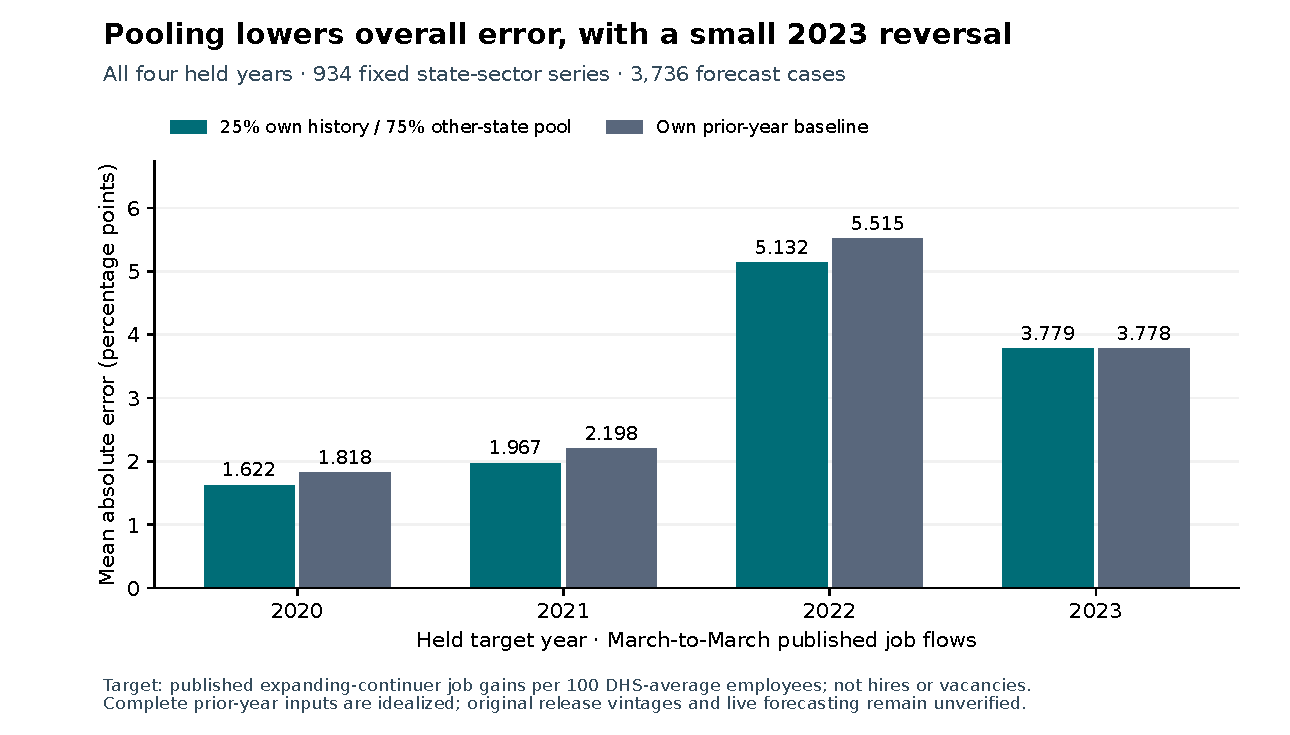
\includegraphics[width=.97\linewidth]{images/year_errors.pdf}\end{center}
\small Figure 1. Every held year is retained. 2022 has the largest error, and 2023 is a small selected-model reversal. Annual BDS flows are March-to-March; the chart does not establish the cause of temporal changes.\normalsize\par

\newpage\section*{1. Captured source and fixed predictor}
The official 2023 BDS State by Sector release [1,2] contains 44,574 rows. The public projection retains fifteen factual key/count/denominator fields in 13,566 state-sector/year rows for 2010--2023. It covers fifty states plus DC and nineteen 2017-NAICS sectors; Puerto Rico is separate. Full source CSV and manuals remain private. Standard CSV versus a separate pandas C-parser matches 668,610 selected source scalars; independent SQLite count/scaled-sum controls match 336 scalars. Source SHA and bounded before/after header/size/Last-Modified checks are retained.

A series enters the baseline cohort only with six valid 2010--2015 direct continuer-creation counts and a supplied denominator at least 1,000 each year. The fixed cohort contains 934 of 969 state-sector series; thirty-five fail the baseline quality/size screen. Flags and unknowns remain explicit. No suppressed continuer count is reconstructed from a total and birth count. All 3,736 validation and 3,736 held forecast cases have valid inputs/targets under these rules; the complete input/label eligibility tables are retained.

The target uses the directly published continuer-job gain count and supplied DHS-average employment denominator [2]. Continuing-establishment job gains describe expanding establishments; they do not capture all worker changes [4,5]. Do not rebuild the denominator from adjacent aggregate employment cells: ownership/classification changes can alter the grouped population [3]. BLS definitions inform interpretation; no incompatible BLS quarterly data are joined.

\[r_{s,k,t}=100\frac{J^{\mathrm{cont}}_{s,k,t}}{D_{s,k,t}},\qquad \widehat r_{s,k,t}=\lambda r_{s,k,t-1}+(1-\lambda)\frac{100\sum_{u\ne s}J^{\mathrm{cont}}_{u,k,t-1}}{\sum_{u\ne s}D_{u,k,t-1}}.\]
Donors are other baseline-cohort states in the same sector with valid prior-year direct counts and denominators; at least five are required. The target state is excluded from the donor pool. All model inputs come from t-1 under the explicitly idealized availability assumption. No current-year target enters the predictor. Candidate own-history weights are 0, 1/4, 1/2, 3/4 and 1. The own-lag endpoint is the simple baseline; no optimizer, complex machine learning or Bayesian fitting is used.

Choose one global weight by first averaging absolute errors within each series in validation years 2016--2019, then equally across series. Exact score ties prefer smaller own-history weight. Twenty-six dependencies, including the selected 1/4 weight and independent checker, were frozen at f67eb80 before 2020--2023 held summaries. Source inputs/quality were visible without blinding. This is chronological calculation on a later revised release, not verified historical real-time forecasting.

\newpage\section*{2. Complete validation and held comparisons}
All five candidates are retained. MAE, RMSE and denominator-weighted MAE use percentage-point units; MSE uses squared percentage points. Validation contains 3,736 cases and 934 series for every candidate. The selection objective is equal-series MAE, not the secondary denominator-weighted measure.

\begin{center}\small\setlength{\tabcolsep}{4pt}
\begin{tabular}{lrrrr}\toprule
Own weight & MAE & MSE & RMSE & Weighted MAE \\
\midrule
0 & 1.788843 & 7.159998 & 2.675817 & 1.152882 \\
1/4 & 1.722490 & 6.887452 & 2.624396 & 1.102038 \\
1/2 & 1.728513 & 7.341322 & 2.709487 & 1.098912 \\
3/4 & 1.814480 & 8.521606 & 2.919179 & 1.150813 \\
1 & 1.967781 & 10.428304 & 3.229288 & 1.245183 \\
\bottomrule\end{tabular}\end{center}
Held overall comparison: the 1/4 weight remains fixed. Both models use the same 3,736 cases and 934 series; no held choice is made.

\begin{center}\small\setlength{\tabcolsep}{4pt}
\begin{tabular}{lrrrr}\toprule
Model & MAE & MSE & RMSE & Weighted MAE \\
\midrule
Selected 1/4 & 3.124807 & 21.611910 & 4.648861 & 2.546230 \\
Own lag 1 & 3.327210 & 26.275404 & 5.125954 & 2.667888 \\
\bottomrule\end{tabular}\end{center}
\begin{center}\small\setlength{\tabcolsep}{4pt}
\begin{tabular}{rrrrr}\toprule
Year & Cases & Selected MAE & Baseline MAE & Difference \\
\midrule
2020 & 934 & 1.621557 & 1.818040 & -0.196483 \\
2021 & 934 & 1.966621 & 2.198047 & -0.231426 \\
2022 & 934 & 5.132117 & 5.515111 & -0.382995 \\
2023 & 934 & 3.778933 & 3.777642 & 0.001291 \\
\bottomrule\end{tabular}\end{center}
Difference is selected minus baseline: positive means worse. The three fixed prior-denominator subsets below retain the same frozen model. They change the reporting population, and do not establish a validated staffing threshold or recover a suppressed cell.

\begin{center}\small\setlength{\tabcolsep}{4pt}
\begin{tabular}{rrrrrr}\toprule
Prior denom at least & Cases & Series & Selected MAE & Baseline MAE & Difference \\
\midrule
1000 & 3732 & 933 & 3.124485 & 3.325703 & -0.201217 \\
5000 & 3455 & 867 & 3.082839 & 3.250796 & -0.167956 \\
25000 & 2559 & 648 & 2.812255 & 2.941076 & -0.128821 \\
\bottomrule\end{tabular}\end{center}
Score representation is fixed before validation at twelve decimal places in percentage-point units, nearest/ties-to-even. Each target and prediction is computed from exact source rationals, then quantized before scoring. Exact losses refer to those exported decimal values; per-case absolute loss differs from the same unrounded values by at most one trillionth of a percentage point. This computational precision is not source measurement precision. RMSE uses a deterministic decimal square root for display.

\newpage\section*{3. Every held sector}
The overall result does not apply uniformly. The complete nineteen-sector display uses equal-series MAE within each sector; all state-sector series remain available underneath. A higher selected-model error is retained for transport/warehousing, education, arts/recreation and accommodation/food.

\begin{center}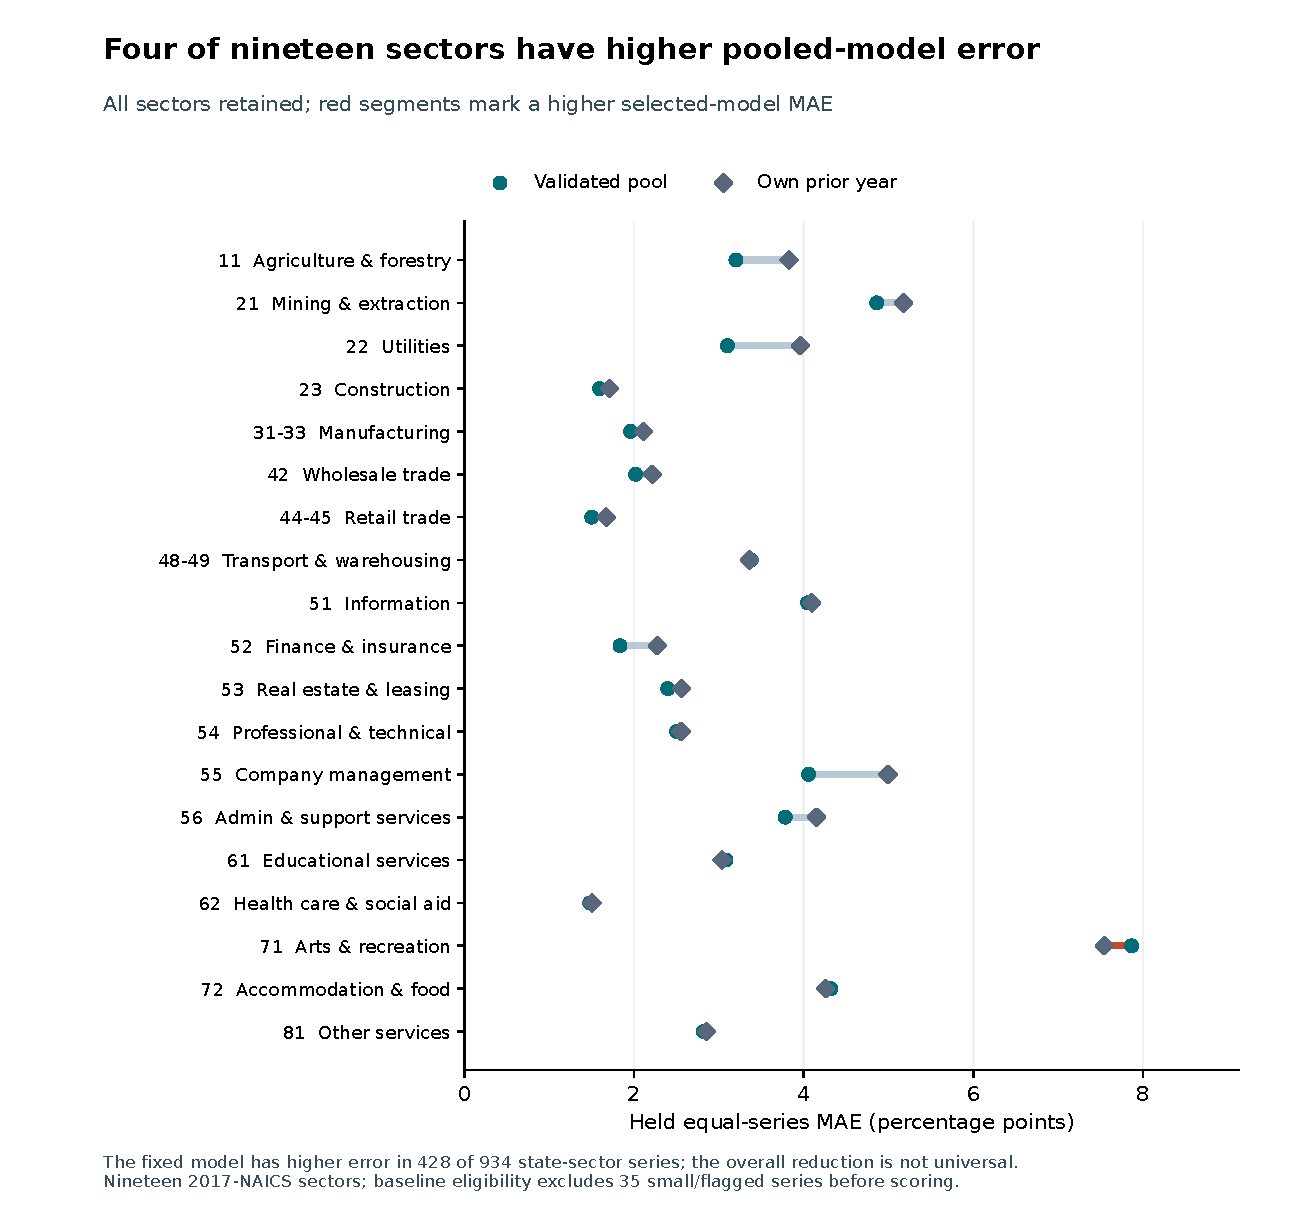
\includegraphics[width=.94\linewidth]{images/sector_errors.pdf}\end{center}
\small Figure 2. Every sector is shown, including four higher-error selected-model cases. Red segments are a sign cue; both actual point values and all paired losses are retained. The cohort does not represent all employers or current hiring.\normalsize\par

\newpage\section*{4. Sector and local failure tables}
\begin{center}\small\setlength{\tabcolsep}{4pt}
\begin{tabular}{llrrrr}\toprule
Sector & Short label & Series & Selected MAE & Baseline MAE & Difference \\
\midrule
11 & Agriculture/forestry & 31 & 3.200861 & 3.829193 & -0.628331 \\
21 & Mining/extraction & 39 & 4.862585 & 5.177612 & -0.315026 \\
22 & Utilities & 50 & 3.101715 & 3.960264 & -0.858550 \\
23 & Construction & 51 & 1.592864 & 1.709688 & -0.116824 \\
31-33 & Manufacturing & 50 & 1.959406 & 2.110424 & -0.151019 \\
42 & Wholesale & 51 & 2.018314 & 2.215880 & -0.197566 \\
44-45 & Retail & 51 & 1.500814 & 1.671365 & -0.170551 \\
48-49 & Transport/warehousing & 51 & 3.378581 & 3.359554 & 0.019027 \\
51 & Information & 51 & 4.046648 & 4.095743 & -0.049094 \\
52 & Finance/insurance & 51 & 1.834795 & 2.274995 & -0.440199 \\
53 & Real estate/leasing & 51 & 2.397177 & 2.559551 & -0.162374 \\
54 & Professional/technical & 51 & 2.500913 & 2.555661 & -0.054748 \\
55 & Company management & 50 & 4.058407 & 4.996047 & -0.937640 \\
56 & Admin/support & 51 & 3.783324 & 4.150698 & -0.367374 \\
61 & Education & 51 & 3.083902 & 3.037646 & 0.046256 \\
62 & Health/social assistance & 51 & 1.478447 & 1.505938 & -0.027491 \\
71 & Arts/recreation & 51 & 7.867361 & 7.545962 & 0.321398 \\
72 & Accommodation/food & 51 & 4.320455 & 4.261589 & 0.058865 \\
81 & Other services & 51 & 2.818479 & 2.852701 & -0.034222 \\
\bottomrule\end{tabular}\end{center}
Of 934 state-sector series, 506 have lower selected-model MAE and 428 have higher MAE; none ties. The five largest higher-error differences below are descriptive examples selected after evaluation, not a model-selection or inference procedure. The complete 934-series comparison is retained in the result CSV.

\begin{center}\small\setlength{\tabcolsep}{4pt}
\begin{tabular}{lrrr}\toprule
State FIPS | sector & Selected MAE & Baseline MAE & Difference \\
\midrule
56|71 & 4.429363 & 1.535492 & 2.893871 \\
40|71 & 6.027131 & 3.482660 & 2.544471 \\
32|21 & 4.074591 & 1.809710 & 2.264881 \\
44|55 & 3.834174 & 1.754246 & 2.079928 \\
56|21 & 5.873542 & 3.793945 & 2.079597 \\
\bottomrule\end{tabular}\end{center}
A favorable aggregate loss can coexist with material local errors. Do not deploy the common weight to a particular state/industry solely because the overall score improves. Obtain dated inputs and a new prospectively specified evaluation for that decision. The tests here establish only this finite captured-cell benchmark.

\newpage\section*{5. Opening activity and continuing expansion}
Published total job creation combines opening establishments and expansion at continuing establishments. The components answer different questions. Figure 3 uses directly published components on the same complete-component case set within each sector; unavailable components remain unavailable. Summed annual counts across years do not count unique people.

\begin{center}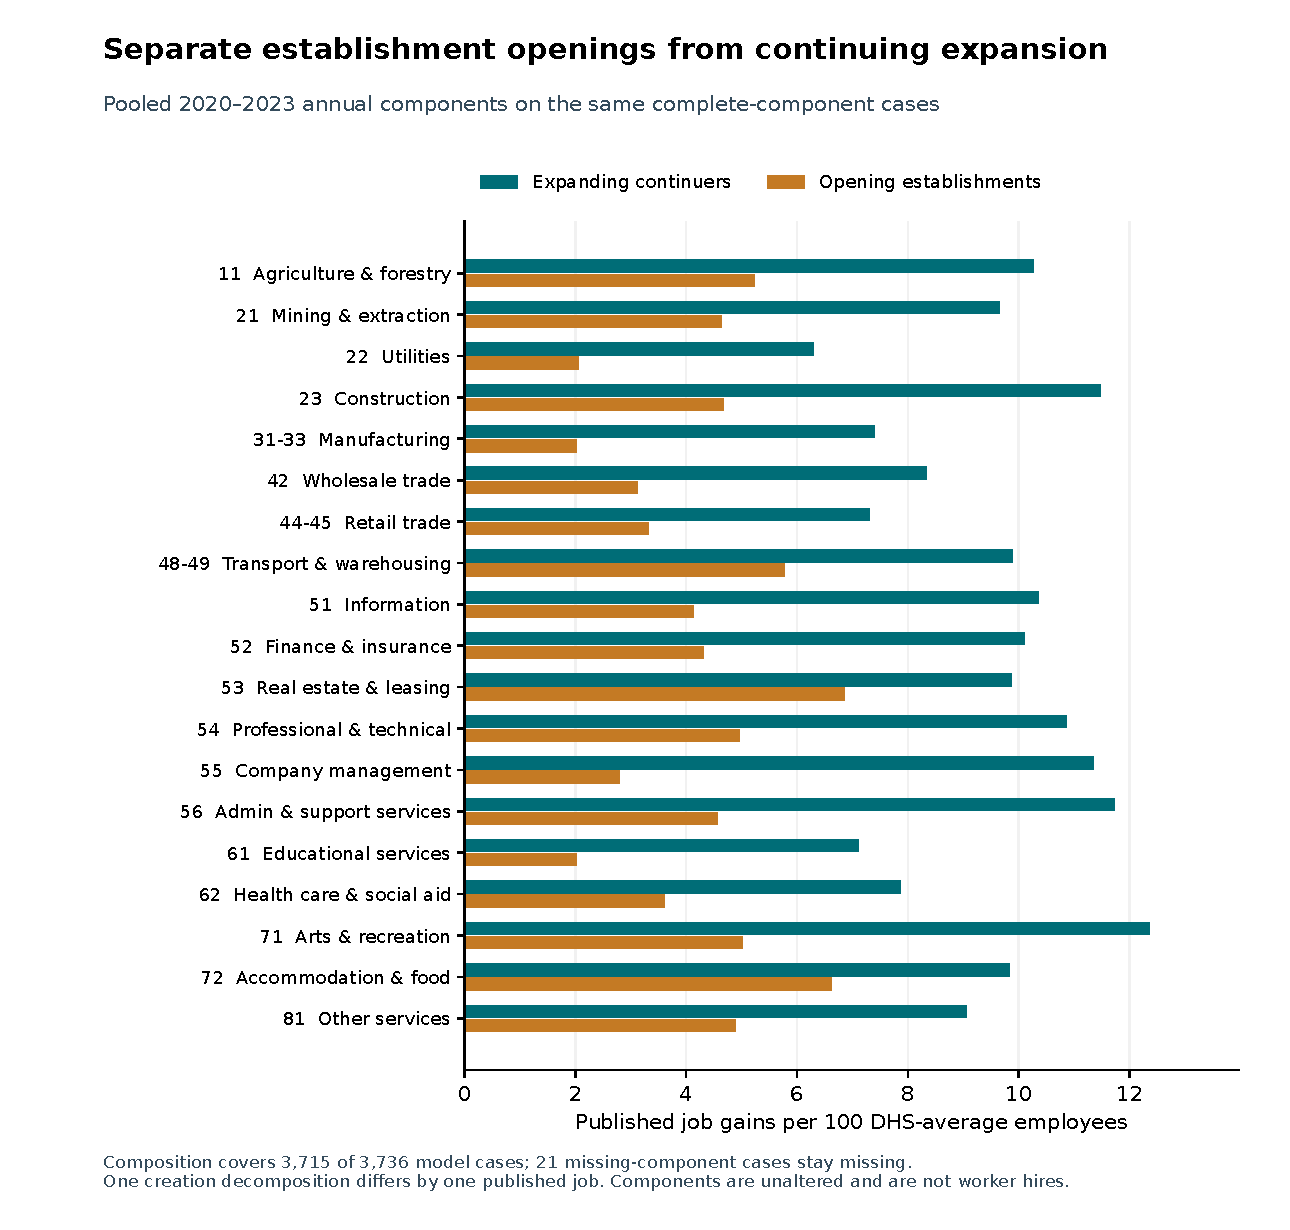
\includegraphics[width=.94\linewidth]{images/creation_components.pdf}\end{center}
\small Figure 3. Separate component bars do not force additivity. Composition covers 3,715 of 3,736 model cases; twenty-one lack a required component. One complete published creation decomposition differs by one job and is left unchanged. These rates are not worker-hire or vacancy rates.\normalsize\par

\newpage\section*{6. Complete composition and disclosure accounting}
Component rates pool the numerator and supplied DHS denominator over complete-component held cases in each sector. Cases and complete cases are shown explicitly. Birth and continuer rates are job gains per 100 reported DHS-average employees. The last columns retain the number and largest absolute size of nonzero published creation-decomposition residuals.

\begin{center}\small\setlength{\tabcolsep}{4pt}
\begin{tabular}{rrrrrrr}\toprule
Sector & Model cases & Complete & Birth rate & Continuer rate & Nonzero & Max jobs \\
\midrule
11 & 124 & 124 & 5.239501 & 10.259712 & 0 & 0 \\
21 & 156 & 153 & 4.638375 & 9.651229 & 0 & 0 \\
22 & 200 & 183 & 2.051356 & 6.290245 & 0 & 0 \\
23 & 204 & 204 & 4.674487 & 11.475035 & 1 & 1 \\
31-33 & 200 & 200 & 2.017553 & 7.397835 & 0 & 0 \\
42 & 204 & 204 & 3.118291 & 8.333612 & 0 & 0 \\
44-45 & 204 & 204 & 3.326205 & 7.316031 & 0 & 0 \\
48-49 & 204 & 204 & 5.776571 & 9.895691 & 0 & 0 \\
51 & 204 & 204 & 4.129926 & 10.355117 & 0 & 0 \\
52 & 204 & 204 & 4.306965 & 10.103031 & 0 & 0 \\
53 & 204 & 204 & 6.860276 & 9.871472 & 0 & 0 \\
54 & 204 & 204 & 4.966372 & 10.855810 & 0 & 0 \\
55 & 200 & 199 & 2.797059 & 11.351910 & 0 & 0 \\
56 & 204 & 204 & 4.571542 & 11.735687 & 0 & 0 \\
61 & 204 & 204 & 2.016931 & 7.108247 & 0 & 0 \\
62 & 204 & 204 & 3.616274 & 7.865248 & 0 & 0 \\
71 & 204 & 204 & 5.022153 & 12.357128 & 0 & 0 \\
72 & 204 & 204 & 6.631142 & 9.832129 & 0 & 0 \\
81 & 204 & 204 & 4.896385 & 9.058715 & 0 & 0 \\
\bottomrule\end{tabular}\end{center}
The 21 excluded composition cases remain in the model evaluation when their directly published target/input is valid. No hidden birth count is inferred from total minus continuer counts. The source quality/disclosure/structural/unavailable tokens remain in the minimal input projection, with their full token inventory. Destruction and net-creation residuals are also retained per cell; no discrepancy is silently forced to zero.

The public BDS release is disclosure protected and historically revised. The general methodology page is explicitly marked no longer current while Census considers alternative protection approaches [3]. This study describes the captured 2023 release and its release-specific codebook; it does not claim that historic noise procedures describe every current or future release. Source truth, true employer-level activity and full labor-market coverage remain unknown. No microdata, employer identities or suppression recovery are used.

\newpage\section*{7. Verification, interpretation and sources}
Sixteen hand-calculated and boundary fixtures pass, including exact ties-to-even quantization, pool endpoints, unequal series/case weighting, zero denominators and suppressed counts. The independent checker imports no model/metric helper: it reconstructs baseline cohorts, lag eligibility and leave-one-state-out donors with SQLite, and reconstructs predictions/selection/losses with rational and independent decimal arithmetic. Validation checks cover 283,484 exact exported fields and 196,792 lineage checks; held checks cover 197,891 fields and 196,792 lineage checks. Isolated replay matches 476,500 exact CSV fields plus five selection/summary/verification documents and all 26 protected dependencies.

The first independent SQL checker stopped on a missing keyword separator; the failed code is retained privately and the targeted correction changed no source, model or result. All three figures were visually inspected and pass 84 plotted-value checks, 114 coordinate/segment checks, eight year annotations, nineteen sector labels and nine export hashes. These finite checks and page inspection do not establish universal correctness, scientific novelty or accessibility conformance.

The target is a published expansion-rate proxy: job gains at expanding continuing establishments per 100 DHS-average employees in the whole state-sector cell. It is not worker hires, job vacancies or a demonstrated labor shortage. This is a retrospective revised-data comparison; complete prior-year inputs are idealized and original information vintages remain unverified.

Use the pooled model as a benchmark candidate, with its own-lag alternative and local failure record visible. Show opening and continuer components separately, preserve unavailable cells and verify dated release availability before an operational forecast. Current hiring or staffing decisions require timely vacancy, worker-flow and business evidence.

\small
1. Census, 2023 BDS public datasets\par\url{https://www.census.gov/data/datasets/time-series/econ/bds/bds-datasets.html}\par
2. Census, 2023-release variable and code definitions\par\url{https://www.census.gov/content/dam/Census/programs-surveys/business-dynamics-statistics/codebook-glossary.pdf}\par
3. Census, methodology and current guidance notice\par\url{https://www.census.gov/programs-surveys/bds/documentation/methodology.html}\par
4. BLS, Job creation and destruction within Washington and Baltimore (2001)\par\url{https://www.bls.gov/opub/mlr/2001/09/art3full.pdf}\par
5. Davis, Haltiwanger and Schuh, Job Creation and Destruction (1996)\par\url{https://mitpress.mit.edu/9780262041522/job-creation-and-destruction/}\par
6. Census public-access rights and citation scope\par\url{https://www2.census.gov/foia/ds_policies/ds027.pdf}\par
\normalsize\par
Scope: Python/SQL annual partial pooling and source composition only. No R execution, quarterly timing, change-point model, new estimator, causal effect, realized savings or exhaustive novelty claim. Reviewed independent manuscripts may be public; formal-publication projects including Azure optimization remain private. Full outputs, exclusions, source hashes and executable checks are in the repository.

\end{document}
